\section{Momentenregelung des Antriebstranges} \label{regelung}

\subsection{Regelungsziele und Regelkreis}
Bevor eine Regelung für die WEA umgesetzt werden kann, müssen zunächst einige Regelungsziele festgelegt werden. Aus der Beschreibung der Regelungsziele ergeben sich die Regelgrößen der WEA. Des Weiteren wird die Komplexität des Reglers durch ein geeignetes Funktionsmodell, welches das dynamische Verhalten der Regelstrecke bestimmt, beschrieben. Hierfür wird das torsionsstarre Triebstrangmodell verwendet. Die Regelung konzentiert sich auf die Einhaltung und Umsetzung der Hauptziele, wobei das Verhalten der Blätter, des Turms und des Antriebsstranges nicht berücksichtigt wird. Folglich reicht ein sehr vereinfachtes Funktionsmodell aus. Die folgende Auflistung fasst die Hauptziele des Reglers zusammen.
\\

Hauptziele:
\begin{enumerate}
    \item Leistungsoptimierung - Leistungsbeiwert \acs{cP} stets auf Maximalwert halten.
    \item Leistungsbegrenzung - Leistungsbeiwert \acs{cP} für eine konstante Entnahme der Nennwindleistung beeinflussen.
\end{enumerate}



Für die Regelung der WEA wird von einem Standardregelkreis ausgegangen, wie in Abbildung 4.1 dargestellt. Als Stellgröße u eignet sich das Generatormoment \acs{MG} und der Pitchwinkel \acs{ThetaP}. Da die Windgeschwindigkeit nur sehr ungenau messtechnisch erfasst werden kann und ein stochastisches Verhalten aufweist, eigenet sich diese Größe als Störgröße z. Hingegen kann die Rotordrehlzahl \acs{omegaR} sehr gut messtechnisch erfasst und verglichen werden und eignet sich daher gut als Führungs- und Regelgröße w und y. Die Regler- und Streckenübertragungsfunktion werden separat mithilfe der Superposition ermittelt. Aus der Generatorcharakteristik lassen sich insgesamt drei Arbeitsbereiche ermitteln, nämlich der untere und obere Teillastbereich, sowie der Volllastbereich. Wobei für den unteren und oberen Teillastbereich eine Leistungsoptimierung vorzusehen ist und für den Volllastbereich eine Leistungsbegrenzung. Auf Grundlage dessen, werden in den folgenden Kapiteln die benötigten Regler für die verschiedenen Arbeitsbereiche und Anforderungen entwickelt. 

\begin{figure}[H]
    \centering
    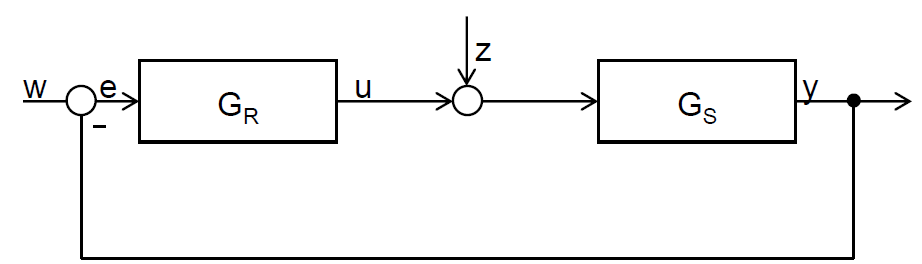
\includegraphics[scale=0.45]{Bilder/Kapitel 6/Standardregelkreis.PNG}
    \caption{Standardregelkreis}
    \label{fig:Standardregelkreis}
\end{figure}
\newpage

\subsection{Unterer Teillastbereich}

Wie bereits erwähnt, ist für den unteren Teillastbereich eine Leistungsoptimierung notwendig, da die Windleistung \acs{PW} unterhalb der Generatornennleistung \acs{PG} liegt. Die Drehzahl \textit{n} liegt folglich noch unter der Generatornenndrehzahl \acs{nG}, wodurch diese noch variabel an die Windgeschwindigkeit \acs{v1} angepasst werden kann. Aufgrund dessen ergibt sich ein optimales Anströmverhältnis und es resultiert ein maximaler Leistungsbeiwert. Im unteren Teillastbereich kann mit steigender Windgeschwindigkeit also die maximal mögliche Windleistung entnommen werden, das heißt, der Leistungsbeiwert \acs{cP} wird stets auf den maximalen Leistungsbeiwert \acs{cPmax} geregelt.


\subsection{Linearisierung der Streckenübertragungsfunktion}

\subsection{Oberer Teillastbereich}
%Einleitung für das Kapitel in Vorlesungsfolie "Einführung in die WEA Regelung" Seite 55
\subsection{Volllastbereich}
%Einleitung für das Kapitel in Vorlesungsfolie "Einführung in die WEA Regelung" Seite 56